% !Rnw weave = knitr
% Writeup of results
% master file

%%%%%%%%%%%%%%%%%%%%%%%%%%
% preamble
%%%%%%%%%%%%%%%%%%%%%%%%%%

% define document class
\documentclass{article}\usepackage{graphicx, color}
%% maxwidth is the original width if it is less than linewidth
%% otherwise use linewidth (to make sure the graphics do not exceed the margin)
\makeatletter
\def\maxwidth{ %
  \ifdim\Gin@nat@width>\linewidth
    \linewidth
  \else
    \Gin@nat@width
  \fi
}
\makeatother

\IfFileExists{upquote.sty}{\usepackage{upquote}}{}
\definecolor{fgcolor}{rgb}{0.2, 0.2, 0.2}
\newcommand{\hlnumber}[1]{\textcolor[rgb]{0,0,0}{#1}}%
\newcommand{\hlfunctioncall}[1]{\textcolor[rgb]{0.501960784313725,0,0.329411764705882}{\textbf{#1}}}%
\newcommand{\hlstring}[1]{\textcolor[rgb]{0.6,0.6,1}{#1}}%
\newcommand{\hlkeyword}[1]{\textcolor[rgb]{0,0,0}{\textbf{#1}}}%
\newcommand{\hlargument}[1]{\textcolor[rgb]{0.690196078431373,0.250980392156863,0.0196078431372549}{#1}}%
\newcommand{\hlcomment}[1]{\textcolor[rgb]{0.180392156862745,0.6,0.341176470588235}{#1}}%
\newcommand{\hlroxygencomment}[1]{\textcolor[rgb]{0.43921568627451,0.47843137254902,0.701960784313725}{#1}}%
\newcommand{\hlformalargs}[1]{\textcolor[rgb]{0.690196078431373,0.250980392156863,0.0196078431372549}{#1}}%
\newcommand{\hleqformalargs}[1]{\textcolor[rgb]{0.690196078431373,0.250980392156863,0.0196078431372549}{#1}}%
\newcommand{\hlassignement}[1]{\textcolor[rgb]{0,0,0}{\textbf{#1}}}%
\newcommand{\hlpackage}[1]{\textcolor[rgb]{0.588235294117647,0.709803921568627,0.145098039215686}{#1}}%
\newcommand{\hlslot}[1]{\textit{#1}}%
\newcommand{\hlsymbol}[1]{\textcolor[rgb]{0,0,0}{#1}}%
\newcommand{\hlprompt}[1]{\textcolor[rgb]{0.2,0.2,0.2}{#1}}%

\usepackage{framed}
\makeatletter
\newenvironment{kframe}{%
 \def\at@end@of@kframe{}%
 \ifinner\ifhmode%
  \def\at@end@of@kframe{\end{minipage}}%
  \begin{minipage}{\columnwidth}%
 \fi\fi%
 \def\FrameCommand##1{\hskip\@totalleftmargin \hskip-\fboxsep
 \colorbox{shadecolor}{##1}\hskip-\fboxsep
     % There is no \\@totalrightmargin, so:
     \hskip-\linewidth \hskip-\@totalleftmargin \hskip\columnwidth}%
 \MakeFramed {\advance\hsize-\width
   \@totalleftmargin\z@ \linewidth\hsize
   \@setminipage}}%
 {\par\unskip\endMakeFramed%
 \at@end@of@kframe}
\makeatother

\definecolor{shadecolor}{rgb}{.97, .97, .97}
\definecolor{messagecolor}{rgb}{0, 0, 0}
\definecolor{warningcolor}{rgb}{1, 0, 1}
\definecolor{errorcolor}{rgb}{1, 0, 0}
\newenvironment{knitrout}{}{} % an empty environment to be redefined in TeX

\usepackage{alltt}

% get required packages
\usepackage{graphicx}   % for graphics
\usepackage{mathtools}  % for math formulas
\usepackage{amssymb}    % for more math styles
\usepackage{amsfonts}    % for more math styles
%\usepackage{amsmath}
%\usepackage[retainorgcmds]{IEEEtrantools}   % advanced equation alignment
\usepackage{makeidx}    % for index generation
%\usepackage{multind}
\usepackage{showidx}

% we are using primarily png graphics
\DeclareGraphicsExtensions{.png}

% make an index
\makeindex

% Title of book
\newcommand{\myTitle}{Valid Inference from Early Stage Surveys}

% This puts the chapter name at the top of the page
\pagestyle{headings}

   % generate concordance
   % images are .45*linewidth by default and are png by default
   % background color of code chunks.




\title{\myTitle}
\author{Richard Garfield\\ Columbia University School of Nursing \and Jared P. Lander\\ JP Lander Consulting}

%%%%%%%%%%%%%%%%%%%%%%%%%%
% the main document
%%%%%%%%%%%%%%%%%%%%%%%%%%
\begin{document}
%\frontmatter    % beginning of book
\maketitle      % create the title page
\tableofcontents    % table of contents


% bulk of the book
%\mainmatter
\section{Distribution Functions}
\label{sec:DistributionFunctions}
These are the functions used to calculate the distribution of each answer. They are general and should workd with any question.

\begin{knitrout}
\definecolor{shadecolor}{rgb}{1, 1, 1}\color{fgcolor}\begin{kframe}
\begin{alltt}
\hlcomment{# Distribution functions}
\hlfunctioncall{require}(useful)
\hlcomment{## builds the distribution for a given question}
build.dist <- \hlfunctioncall{function}(data, lhs, group, question) \{
    theFormula <- \hlfunctioncall{build.formula}(lhs = lhs, rhs = \hlfunctioncall{c}(group, question))
    agg <- \hlfunctioncall{aggregate}(theFormula, data, length)
    agg <- \hlfunctioncall{ddply}(agg, .variables = group, .fun = \hlfunctioncall{function}(x) \{
        x$Percent <- x[[lhs]]/\hlfunctioncall{sum}(x[[lhs]])
        \hlfunctioncall{return}(x)
    \})
    agg
\}


\hlcomment{## get random Tehsils from a province}
village.list <- \hlfunctioncall{function}(x, num = 5, unit = \hlstring{"Tehsil"}) \{
    \hlcomment{# get list of units}
    units <- \hlfunctioncall{unique}(x[, unit])
    
    \hlcomment{# sample num of those without replacement}
    keepers <- \hlfunctioncall{sample}(x = units, size = \hlfunctioncall{min}(num, \hlfunctioncall{length}(units)), replace = FALSE)
    
    \hlfunctioncall{return}(\hlfunctioncall{as.character}(keepers))
\}


\hlcomment{# function to make names of dist's better}
change.names <- \hlfunctioncall{function}(names, include = names, prefix = \hlstring{""}) \{
    theOnes <- \hlfunctioncall{which}(!names %in% include)
    names[theOnes] <- \hlfunctioncall{sprintf}(\hlstring{"%s.%s"}, prefix, names[theOnes])
    \hlfunctioncall{return}(names)
\}

\hlcomment{## function to impute missing}
impute.col <- \hlfunctioncall{function}(col, value = 0) \{
    col[\hlfunctioncall{is.na}(col)] <- value
    \hlfunctioncall{return}(col)
\}

\hlcomment{## this compares two distributions and computes an MSE}
compare.dist <- \hlfunctioncall{function}(full, partial, compare = \hlstring{"Percent"}, by = \hlfunctioncall{intersect}(\hlfunctioncall{names}(full), 
    \hlfunctioncall{names}(partial))) \{
    \hlcomment{# prepend Pull onto certain names in full}
    \hlfunctioncall{names}(full) <- \hlfunctioncall{change.names}(names = \hlfunctioncall{names}(full), include = by, prefix = \hlstring{"Full"})
    
    \hlcomment{# prepend Partial onto certain names in full}
    \hlfunctioncall{names}(partial) <- \hlfunctioncall{change.names}(names = \hlfunctioncall{names}(partial), include = by, prefix = \hlstring{"Partial"})
    
    full.compare <- \hlfunctioncall{sprintf}(\hlstring{"Full.%s"}, compare)
    partial.compare <- \hlfunctioncall{sprintf}(\hlstring{"Partial.%s"}, compare)
    
    \hlcomment{# join the two together}
    both <- \hlfunctioncall{join}(x = full, y = partial, by = by, type = \hlstring{"left"})
    
    \hlfunctioncall{rm}(full, partial)
    
    \hlcomment{## fill in any NA's with zero}
    both[[full.compare]] <- \hlfunctioncall{impute.col}(col = both[[full.compare]], value = 0)
    both[[partial.compare]] <- \hlfunctioncall{impute.col}(col = both[[partial.compare]], value = 0)
    
    both$.Diff <- both[[full.compare]] - both[[partial.compare]]
    
    both$.MSE <- \hlfunctioncall{mean}(both$.Diff^2)
    
    \hlcomment{# \hlfunctioncall{attr}(x=both, which=\hlstring{'MSE'}) <- \hlfunctioncall{mean}(both$.Diff^2)}
    
    \hlcomment{# \hlfunctioncall{aggregate}(\hlfunctioncall{build.formula}(lhs=\hlstring{'.Diff'}, rhs=}
    
    \hlfunctioncall{return}(both)
\}
\end{alltt}
\end{kframe}
\end{knitrout}


% !Rnw weave = knitr
% Initial stuff
\section{Initial Stuff}
\label{sec:initial}
The data is as described in Section ~\ref{sec:thedata}.

We examined the answer to the question``What percentage of rice crops were lost due to the flood?''  We then randomly chose five Tehsils from each province, then 10, then 15 and performed the same analysis on the reduced data.

In situations where a province has fewer than five, 10 or 15 Tehsils sampled, all were used.
Small change

% !Rnw weave = knitr
% The Data
\section{The Data}
\label{sec:thedata}


The data was collected following the floods in Pakistan in 2010. Small Changes.

It surveyed affected villages in GB, KPK, Punjab and Sindh.

% make code to plot Vill distribution but don't run or show it.



The distribution of villages within Tehsils within Provinces is seen in Figure~\ref{fig:VillageDist}.

\begin{figure}[!hbtp]
\begin{knitrout}
\definecolor{shadecolor}{rgb}{1, 1, 1}\color{fgcolor}\begin{kframe}


{\ttfamily\noindent\textcolor{warningcolor}{\#\# Warning: 'opts' is deprecated.\\\#\# Use 'theme' instead.\\\#\# See help("Deprecated")}}

{\ttfamily\noindent\textcolor{warningcolor}{\#\# Warning: 'theme\_text' is deprecated.\\\#\# Use 'element\_text' instead.\\\#\# See help("Deprecated")}}\end{kframe}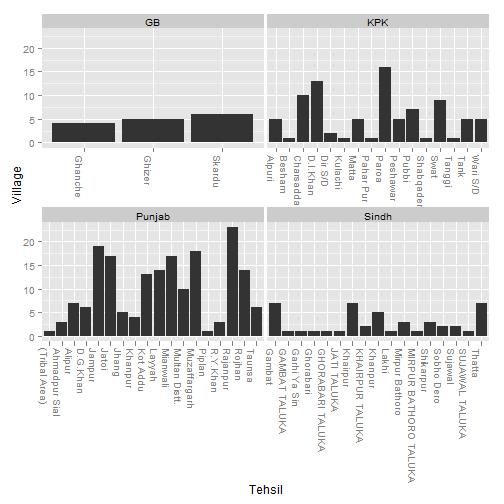
\includegraphics[width=.9\linewidth]{thedata/figures/VillDistPlot} 
\end{knitrout}

\caption{Distribution of villages within Tehsils within the four Provinces.\label{fig:VillageDist}}
\end{figure}

Here is the code to run it.

\begin{knitrout}
\definecolor{shadecolor}{rgb}{1, 1, 1}\color{fgcolor}\begin{kframe}
\begin{alltt}
\hlfunctioncall{ggplot}(vills, \hlfunctioncall{aes}(x = Tehsil)) + \hlfunctioncall{geom_bar}(\hlfunctioncall{aes}(y = Village), stat = \hlstring{"identity"}) + 
    \hlfunctioncall{opts}(axis.text.x = \hlfunctioncall{theme_text}(angle = 270, hjust = 0)) + \hlfunctioncall{facet_wrap}(~Province, 
    scales = \hlstring{"free_x"})
\end{alltt}
\end{kframe}
\end{knitrout}


The analysis begins in Section~\ref{sec:overall}.


\documentclass{article}
\usepackage{knitr}
\newcommand{\SweaveOpts}[1]{}  % do not interfere with LaTeX
\newcommand{\SweaveInput}[1]{} % because they are not real TeX commands
\newcommand{\Sexpr}[1]{}       % will only be parsed by R



% get required packages
\usepackage{graphicx}   % for graphics
\usepackage{mathtools}  % for math formulas
\usepackage{amssymb}    % for more math styles
\usepackage{amsfonts}    % for more math styles
%\usepackage{amsmath}
%\usepackage[retainorgcmds]{IEEEtrantools}   % advanced equation alignment
\usepackage{makeidx}    % for index generation
\usepackage{showidx}

% we are using primarily png graphics
\DeclareGraphicsExtensions{.png,.pdf}

% make an index
\makeindex

% Title of book
\newcommand{\myTitle}{Generalizing from Purposive Surveys\\ How large a Sample is Needed}

% This puts the chapter name at the top of the page
\pagestyle{headings}





\title{\myTitle}
\author{Richard Garfield\\ Columbia University School of Nursing \and Jared P. Lander\\ JP Lander Consulting}

%%%%%%%%%%%%%%%%%%%%%%%%%%
% the main document
%%%%%%%%%%%%%%%%%%%%%%%%%%


\begin{document}
% !Rnw weave = knitr


% The Data
\section{Analyzing All Data}
\label{sec:overall}
Here we analyze all of the data.

First we load the data and view a portion of it. Some more details.

These are the necessary packages.
\begin{knitrout}
\definecolor{shadecolor}{rgb}{1, 1, 1}\color{fgcolor}\begin{kframe}
\begin{alltt}
\hlfunctioncall{require}(useful)
\hlfunctioncall{require}(plyr)
\hlfunctioncall{require}(ggplot2)
\end{alltt}
\end{kframe}
\end{knitrout}


\begin{knitrout}
\definecolor{shadecolor}{rgb}{1, 1, 1}\color{fgcolor}\begin{kframe}
\begin{alltt}
\hlfunctioncall{load}(\hlstring{"../../data/pakistan/pak.rdata"})
\hlfunctioncall{source}(\hlstring{"../../R/distFuncs.r"})
\hlfunctioncall{corner}(pak, c = 15)
\end{alltt}
\begin{verbatim}
  New_ID Age  Sex     Date Province District Tehsil
1   1288  26 Male 29082010      KPK  Shangla Besham
2   1290  30 Male 29082010      KPK  Shangla Besham
3   1370  54 Male 28082010      KPK  Shangla Besham
4   1372  53 Male 28082010      KPK  Shangla Besham
5   1371  64 Male 28082010      KPK  Shangla Besham
         Village Latitude Longitude Total Urban Rural
1 abaseen colony    34.94     72.88  90.6     -  90.6
2 abaseen colony    34.94     72.88  90.6     -  90.6
3 abaseen colony    34.94     72.88  90.6     -  90.6
4 abaseen colony    34.94     72.88  90.6     -  90.6
5 abaseen colony    34.94     72.88  90.6     -  90.6
                                Accommodation
1 Collective centers (school/Public building)
2                                 Host family
3          On the site of the house (Damaged)
4          On the site of the house (Damaged)
5          On the site of the house (Damaged)
  StagnantWater
1           Few
2           Few
3           Few
4          None
5          None
\end{verbatim}
\end{kframe}
\end{knitrout}


Now we build a distribution for all the data and visualize it in Figure~\ref{fig:overallDist} with the code here:.
\begin{knitrout}
\definecolor{shadecolor}{rgb}{1, 1, 1}\color{fgcolor}\begin{kframe}
\begin{alltt}
ricePerc <- \hlfunctioncall{build.dist}(data = pak, lhs = \hlstring{"New_ID"}, group = \hlstring{"Province"}, 
    question = \hlstring{"RiceLost"})
ricePerc$Size <- \hlstring{"All"}
\hlfunctioncall{ggplot}(ricePerc, \hlfunctioncall{aes}(x = RiceLost, y = Percent)) + \hlfunctioncall{geom_bar}(stat = \hlstring{"identity"}) + 
    \hlfunctioncall{facet_wrap}(~Province) + \hlfunctioncall{opts}(axis.text.x = \hlfunctioncall{theme_text}(angle = 90))
\end{alltt}
\end{kframe}\begin{figure}[!hbtp]


{\centering \includegraphics[width=.8\linewidth]{figures/overallDist} 

}

\caption[Graphical view of the distribution of responses for all the data]{Graphical view of the distribution of responses for all the data.\label{fig:overallDist}}
\end{figure}


\end{knitrout}



In Section~\ref{sec:smallerDist} we analyze the distribution of responses for samples of fewer Tehsils.
\end{document}

% smaller samples
\section{Analyzing Smaller Samples}
\label{sec:smallerDist}




We build a similar distribution using just 5 Tehsils (max) per province as seen in Figure~\ref{fig:fiveDist} with the code here:.
\begin{knitrout}
\definecolor{shadecolor}{rgb}{0.969, 0.969, 0.969}\color{fgcolor}\begin{kframe}
\begin{flushleft}
\ttfamily\noindent
\hlsymbol{pak5}{\ }\hlassignement{\usebox{\hlnormalsizeboxlessthan}-}{\ }\hlsymbol{pak}\hlkeyword{[}\hlsymbol{pak}\hlkeyword{\usebox{\hlnormalsizeboxdollar}}\hlsymbol{Tehsil}{\ }\hlkeyword{\usebox{\hlnormalsizeboxpercent}in\usebox{\hlnormalsizeboxpercent}}{\ }\hlfunctioncall{unlist}\hlkeyword{(}\hlfunctioncall{dlply}\hlkeyword{(}\hlsymbol{pak}\hlkeyword{,}{\ }\hlargument{.variables}{\ }\hlargument{=}{\ }\hlstring{"{}Province"{}}\hlkeyword{,}\hspace*{\fill}\\
\hlstd{}{\ }{\ }{\ }{\ }\hlargument{.fun}{\ }\hlargument{=}{\ }\hlsymbol{village.list}\hlkeyword{,}{\ }\hlargument{num}{\ }\hlargument{=}{\ }\hlnumber{5}\hlkeyword{,}{\ }\hlargument{unit}{\ }\hlargument{=}{\ }\hlstring{"{}Tehsil"{}}\hlkeyword{)}\hlkeyword{)}\hlkeyword{,}{\ }\hlkeyword{]}\hspace*{\fill}\\
\hlstd{}\hlsymbol{pak5}\hlkeyword{\usebox{\hlnormalsizeboxdollar}}\hlsymbol{Tehsil}{\ }\hlassignement{\usebox{\hlnormalsizeboxlessthan}-}{\ }\hlfunctioncall{factor}\hlkeyword{(}\hlsymbol{pak5}\hlkeyword{\usebox{\hlnormalsizeboxdollar}}\hlsymbol{Tehsil}\hlkeyword{)}\hspace*{\fill}\\
\hlstd{}\hlsymbol{rice5Perc}{\ }\hlassignement{\usebox{\hlnormalsizeboxlessthan}-}{\ }\hlfunctioncall{build.dist}\hlkeyword{(}\hlargument{data}{\ }\hlargument{=}{\ }\hlsymbol{pak5}\hlkeyword{,}{\ }\hlargument{lhs}{\ }\hlargument{=}{\ }\hlstring{"{}New\usebox{\hlnormalsizeboxunderscore}ID"{}}\hlkeyword{,}{\ }\hlargument{group}{\ }\hlargument{=}{\ }\hlstring{"{}Province"{}}\hlkeyword{,}\hspace*{\fill}\\
\hlstd{}{\ }{\ }{\ }{\ }\hlargument{question}{\ }\hlargument{=}{\ }\hlstring{"{}RiceLost"{}}\hlkeyword{)}\hspace*{\fill}\\
\hlstd{}\hlsymbol{rice5Perc}\hlkeyword{\usebox{\hlnormalsizeboxdollar}}\hlsymbol{Size}{\ }\hlassignement{\usebox{\hlnormalsizeboxlessthan}-}{\ }\hlstring{"{}5"{}}\hspace*{\fill}\\
\hlstd{}\hlsymbol{compare5}{\ }\hlassignement{\usebox{\hlnormalsizeboxlessthan}-}{\ }\hlfunctioncall{compare.dist}\hlkeyword{(}\hlsymbol{ricePerc}\hlkeyword{,}{\ }\hlsymbol{rice5Perc}\hlkeyword{,}{\ }\hlargument{by}{\ }\hlargument{=}{\ }\hlfunctioncall{c}\hlkeyword{(}\hlstring{"{}Province"{}}\hlkeyword{,}\hspace*{\fill}\\
\hlstd{}{\ }{\ }{\ }{\ }\hlstring{"{}RiceLost"{}}\hlkeyword{)}\hlkeyword{)}\hspace*{\fill}\\
\hlstd{}\hlsymbol{compare5}\hlkeyword{\usebox{\hlnormalsizeboxdollar}}\hlsymbol{Partial.Size}{\ }\hlassignement{\usebox{\hlnormalsizeboxlessthan}-}{\ }\hlfunctioncall{impute.col}\hlkeyword{(}\hlargument{col}{\ }\hlargument{=}{\ }\hlsymbol{compare5}\hlkeyword{\usebox{\hlnormalsizeboxdollar}}\hlsymbol{Partial.Size}\hlkeyword{,}\hspace*{\fill}\\
\hlstd{}{\ }{\ }{\ }{\ }\hlnumber{5}\hlkeyword{)}\hspace*{\fill}\\
\hlstd{}\hlfunctioncall{ggplot}\hlkeyword{(}\hlsymbol{rice5Perc}\hlkeyword{,}{\ }\hlfunctioncall{aes}\hlkeyword{(}\hlargument{x}{\ }\hlargument{=}{\ }\hlsymbol{RiceLost}\hlkeyword{,}{\ }\hlargument{y}{\ }\hlargument{=}{\ }\hlsymbol{Percent}\hlkeyword{)}\hlkeyword{)}{\ }\hlkeyword{+}{\ }\hlfunctioncall{geom\usebox{\hlnormalsizeboxunderscore}bar}\hlkeyword{(}\hlargument{stat}{\ }\hlargument{=}{\ }\hlstring{"{}identity"{}}\hlkeyword{)}{\ }\hlkeyword{+}\hspace*{\fill}\\
\hlstd{}{\ }{\ }{\ }{\ }\hlfunctioncall{facet\usebox{\hlnormalsizeboxunderscore}wrap}\hlkeyword{(}\hlkeyword{\urltilda{}}\hlsymbol{Province}\hlkeyword{)}{\ }\hlkeyword{+}{\ }\hlfunctioncall{opts}\hlkeyword{(}\hlargument{axis.text.x}{\ }\hlargument{=}{\ }\hlfunctioncall{theme\usebox{\hlnormalsizeboxunderscore}text}\hlkeyword{(}\hlargument{angle}{\ }\hlargument{=}{\ }\hlnumber{90}\hlkeyword{)}\hlkeyword{)}\mbox{}
\normalfont
\end{flushleft}
\end{kframe}
\end{knitrout}


\begin{figure}[!hbt]
\begin{knitrout}
\definecolor{shadecolor}{rgb}{0.969, 0.969, 0.969}\color{fgcolor}

{\centering 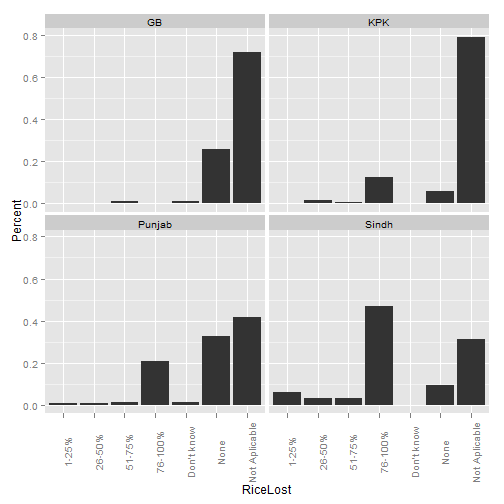
\includegraphics[width=.9\linewidth]{smallerDist/figures/fiveDistPlot} 

}


\end{knitrout}

\caption{Distribution for five Tehsils per Province.\label{fig:fiveDist}}
\end{figure}

The same distributions for 10 and 15 samples are seen in Figures~\ref{fig:tenDist} and \ref{fig:fifteenDist} respectively.  This time, for brevity, the code will not be displayed.

\begin{figure}[!hbt]
\begin{knitrout}
\definecolor{shadecolor}{rgb}{0.969, 0.969, 0.969}\color{fgcolor}

{\centering 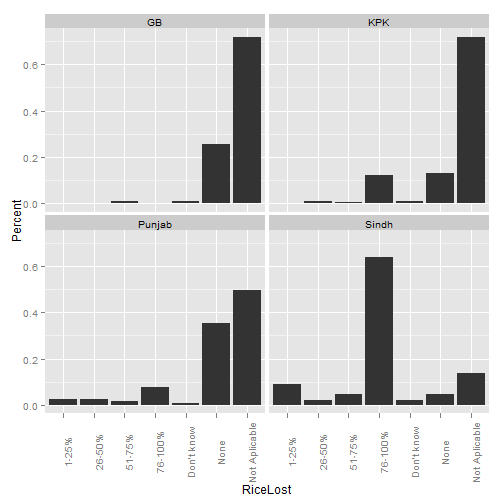
\includegraphics[width=.9\linewidth]{smallerDist/figures/tenDist} 

}


\end{knitrout}

\caption{Distribution for ten Tehsil per Province.\label{fig:tenDist}}
\end{figure}

\begin{figure}[!hbtp]
\begin{knitrout}
\definecolor{shadecolor}{rgb}{0.969, 0.969, 0.969}\color{fgcolor}

{\centering 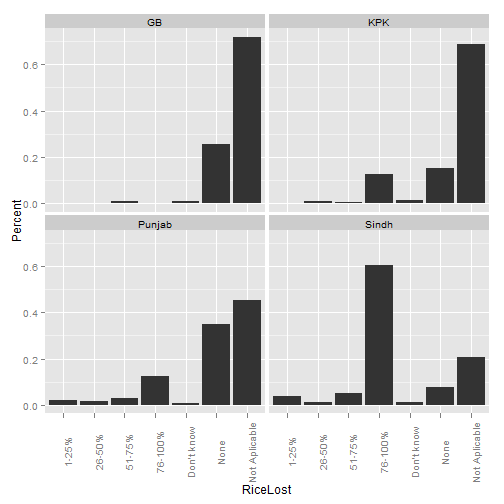
\includegraphics[width=.9\linewidth]{smallerDist/figures/fifteenDist} 

}


\end{knitrout}

\caption{Distribution for 15 Tehsils per Province.\label{fig:fifteenDist}}
\end{figure}

Now we wish to to look at the various distributions in a single plot.  Here is the code:
\begin{knitrout}
\definecolor{shadecolor}{rgb}{0.969, 0.969, 0.969}\color{fgcolor}\begin{kframe}
\begin{flushleft}
\ttfamily\noindent
\hlcomment{\usebox{\hlnormalsizeboxhash}{\ }plot{\ }distributions{\ }for{\ }all{\ }measurement{\ }sizes{\ }on{\ }same{\ }graph}\hspace*{\fill}\\
\hlstd{}\hlsymbol{allT}{\ }\hlassignement{\usebox{\hlnormalsizeboxlessthan}-}{\ }\hlfunctioncall{rbind}\hlkeyword{(}\hlsymbol{rice5Perc}\hlkeyword{,}{\ }\hlsymbol{rice10Perc}\hlkeyword{,}{\ }\hlsymbol{rice15Perc}\hlkeyword{,}{\ }\hlsymbol{ricePerc}\hlkeyword{)}\hspace*{\fill}\\
\hlstd{}\hlsymbol{allT}\hlkeyword{\usebox{\hlnormalsizeboxdollar}}\hlsymbol{Size}{\ }\hlassignement{\usebox{\hlnormalsizeboxlessthan}-}{\ }\hlfunctioncall{ordered}\hlkeyword{(}\hlsymbol{allT}\hlkeyword{\usebox{\hlnormalsizeboxdollar}}\hlsymbol{Size}\hlkeyword{,}{\ }\hlargument{levels}{\ }\hlargument{=}{\ }\hlfunctioncall{c}\hlkeyword{(}\hlnumber{5}\hlkeyword{,}{\ }\hlnumber{10}\hlkeyword{,}{\ }\hlnumber{15}\hlkeyword{,}{\ }\hlstring{"{}All"{}}\hlkeyword{)}\hlkeyword{)}\hspace*{\fill}\\
\hlstd{}\hlfunctioncall{ggplot}\hlkeyword{(}\hlsymbol{allT}\hlkeyword{,}{\ }\hlfunctioncall{aes}\hlkeyword{(}\hlargument{x}{\ }\hlargument{=}{\ }\hlsymbol{RiceLost}\hlkeyword{,}{\ }\hlargument{y}{\ }\hlargument{=}{\ }\hlsymbol{Percent}\hlkeyword{)}\hlkeyword{)}{\ }\hlkeyword{+}{\ }\hlfunctioncall{geom\usebox{\hlnormalsizeboxunderscore}bar}\hlkeyword{(}\hlfunctioncall{aes}\hlkeyword{(}\hlargument{group}{\ }\hlargument{=}{\ }\hlsymbol{Size}\hlkeyword{,}\hspace*{\fill}\\
\hlstd{}{\ }{\ }{\ }{\ }\hlargument{fill}{\ }\hlargument{=}{\ }\hlsymbol{Size}\hlkeyword{)}\hlkeyword{,}{\ }\hlargument{stat}{\ }\hlargument{=}{\ }\hlstring{"{}identity"{}}\hlkeyword{,}{\ }\hlargument{position}{\ }\hlargument{=}{\ }\hlstring{"{}dodge"{}}\hlkeyword{)}{\ }\hlkeyword{+}{\ }\hlfunctioncall{opts}\hlkeyword{(}\hlargument{axis.text.x}{\ }\hlargument{=}{\ }\hlfunctioncall{theme\usebox{\hlnormalsizeboxunderscore}text}\hlkeyword{(}\hlargument{angle}{\ }\hlargument{=}{\ }\hlnumber{90}\hlkeyword{)}\hlkeyword{)}{\ }\hlkeyword{+}\hspace*{\fill}\\
\hlstd{}{\ }{\ }{\ }{\ }\hlfunctioncall{facet\usebox{\hlnormalsizeboxunderscore}wrap}\hlkeyword{(}\hlkeyword{\urltilda{}}\hlsymbol{Province}\hlkeyword{)}\mbox{}
\normalfont
\end{flushleft}
\end{kframe}
\end{knitrout}


The plot is in Figure~\ref{fig:allDistInOne}.
\begin{figure}[!hbtp]
\begin{knitrout}
\definecolor{shadecolor}{rgb}{0.969, 0.969, 0.969}\color{fgcolor}

{\centering 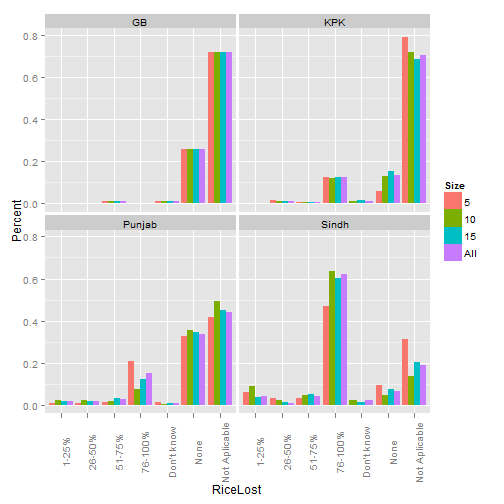
\includegraphics[width=.9\linewidth]{smallerDist/figures/allDistInOnePlot} 

}


\end{knitrout}

\caption{The distribution for all sampling types in one plot.\label{fig:allDistInOne}}
\end{figure}

Figure~\ref{fig:distErrors} displays the error between the smaller samples and the full distribution.  The code to do so is here:

\begin{knitrout}
\definecolor{shadecolor}{rgb}{0.969, 0.969, 0.969}\color{fgcolor}\begin{kframe}
\begin{flushleft}
\ttfamily\noindent
\hlsymbol{allC}{\ }\hlassignement{\usebox{\hlnormalsizeboxlessthan}-}{\ }\hlfunctioncall{rbind}\hlkeyword{(}\hlsymbol{compare5}\hlkeyword{,}{\ }\hlsymbol{compare10}\hlkeyword{,}{\ }\hlsymbol{compare15}\hlkeyword{)}\hspace*{\fill}\\
\hlstd{}\hlsymbol{allC}\hlkeyword{\usebox{\hlnormalsizeboxdollar}}\hlsymbol{Partial.Size}{\ }\hlassignement{\usebox{\hlnormalsizeboxlessthan}-}{\ }\hlfunctioncall{ordered}\hlkeyword{(}\hlsymbol{allC}\hlkeyword{\usebox{\hlnormalsizeboxdollar}}\hlsymbol{Partial.Size}\hlkeyword{,}{\ }\hlargument{levels}{\ }\hlargument{=}{\ }\hlfunctioncall{c}\hlkeyword{(}\hlnumber{5}\hlkeyword{,}{\ }\hlnumber{10}\hlkeyword{,}\hspace*{\fill}\\
\hlstd{}{\ }{\ }{\ }{\ }\hlnumber{15}\hlkeyword{)}\hlkeyword{)}\hspace*{\fill}\\
\hlstd{}\hlsymbol{allC}\hlkeyword{\usebox{\hlnormalsizeboxdollar}}\hlsymbol{Province}{\ }\hlassignement{\usebox{\hlnormalsizeboxlessthan}-}{\ }\hlfunctioncall{factor}\hlkeyword{(}\hlsymbol{allC}\hlkeyword{\usebox{\hlnormalsizeboxdollar}}\hlsymbol{Province}\hlkeyword{)}\hspace*{\fill}\\
\hlstd{}\hlfunctioncall{ggplot}\hlkeyword{(}\hlsymbol{allC}\hlkeyword{,}{\ }\hlfunctioncall{aes}\hlkeyword{(}\hlargument{x}{\ }\hlargument{=}{\ }\hlsymbol{RiceLost}\hlkeyword{,}{\ }\hlargument{y}{\ }\hlargument{=}{\ }\hlsymbol{.Diff}\hlkeyword{)}\hlkeyword{)}{\ }\hlkeyword{+}{\ }\hlfunctioncall{geom\usebox{\hlnormalsizeboxunderscore}line}\hlkeyword{(}\hlfunctioncall{aes}\hlkeyword{(}\hlargument{fill}{\ }\hlargument{=}{\ }\hlsymbol{Province}\hlkeyword{,}\hspace*{\fill}\\
\hlstd{}{\ }{\ }{\ }{\ }\hlargument{colour}{\ }\hlargument{=}{\ }\hlsymbol{Province}\hlkeyword{,}{\ }\hlargument{group}{\ }\hlargument{=}{\ }\hlsymbol{Province}\hlkeyword{)}\hlkeyword{)}{\ }\hlkeyword{+}{\ }\hlfunctioncall{opts}\hlkeyword{(}\hlargument{axis.text.x}{\ }\hlargument{=}{\ }\hlfunctioncall{theme\usebox{\hlnormalsizeboxunderscore}text}\hlkeyword{(}\hlargument{angle}{\ }\hlargument{=}{\ }\hlnumber{90}\hlkeyword{)}\hlkeyword{)}{\ }\hlkeyword{+}\hspace*{\fill}\\
\hlstd{}{\ }{\ }{\ }{\ }\hlfunctioncall{facet\usebox{\hlnormalsizeboxunderscore}wrap}\hlkeyword{(}\hlkeyword{\urltilda{}}\hlsymbol{Partial.Size}\hlkeyword{)}{\ }\hlkeyword{+}{\ }\hlfunctioncall{geom\usebox{\hlnormalsizeboxunderscore}hline}\hlkeyword{(}\hlargument{yintercept}{\ }\hlargument{=}{\ }\hlnumber{0}\hlkeyword{,}{\ }\hlargument{colour}{\ }\hlargument{=}{\ }\hlstring{"{}grey"{}}\hlkeyword{,}\hspace*{\fill}\\
\hlstd{}{\ }{\ }{\ }{\ }\hlargument{linetype}{\ }\hlargument{=}{\ }\hlnumber{2}\hlkeyword{)}\mbox{}
\normalfont
\end{flushleft}
\end{kframe}
\end{knitrout}


\begin{figure}[!hbtp]
\begin{knitrout}
\definecolor{shadecolor}{rgb}{0.969, 0.969, 0.969}\color{fgcolor}

{\centering 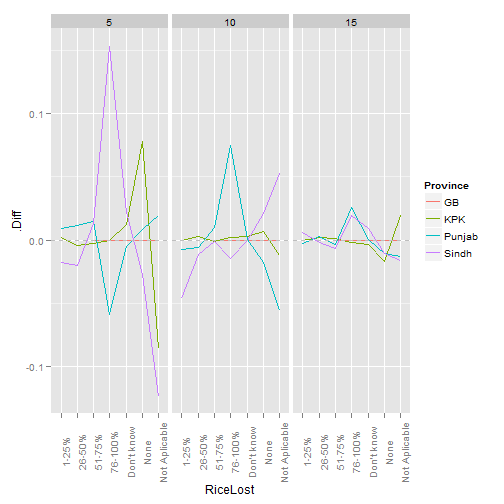
\includegraphics[width=.9\linewidth]{smallerDist/figures/distErrorsPlot} 

}


\end{knitrout}

\caption[Distribution Differences.]{The difference between the true distribution and the smaller smaples.\label{fig:distErrors}}
\end{figure}

Closing text.


%\appendix
%\backmatter
\cleardoublepage
\addcontentsline{toc}{section}{\numberline{}List of Figures}
\listoffigures
%\cleardoublepage
%\listoftables
%\cleardoublepage
\printindex
\end{document}
